\documentclass{beamer}
\beamertemplatenavigationsymbolsempty
\usecolortheme{beaver}
\setbeamertemplate{blocks}[rounded=true, shadow=true]
\setbeamertemplate{footline}[page number]
%
\usepackage[utf8]{inputenc}
\usepackage[english,russian]{babel}
\usepackage{amssymb,amsfonts,amsmath,mathtext}
\usepackage{subfig}
\usepackage[all]{xy} % xy package for diagrams
\usepackage{array}
\usepackage{multicol}% many columns in slide
\usepackage{hyperref}% urls
\usepackage{tabularx}
\usepackage{hhline}%tables
% Your figures are here:
\graphicspath{ {fig/} {../figures/} }
\usepackage{amsmath}
\DeclareMathOperator*{\argmax}{arg\,max}
\DeclareMathOperator*{\argmin}{arg\,min}
%----------------------------------------------------------------------------------------------------------
\title[\hbox to 56mm{Жадный метод оптимизации первого порядка с относительным шумом}]{Жадный метод оптимизации первого порядка с относительным шумом}
\author[Д.\,Н. Рубцов]{Денис Николаевич Рубцов}
\institute{Московский физико-технический институт}
\date{\footnotesize
\par\smallskip\emph{Курс:} Автоматизация научных исследований\par (практика, В.\,В.~Стрижов)/Группа 105
\par\smallskip\emph{Эксперт:} к.ф.-м.н. Э.\,А.~Горбунов
\par\smallskip\emph{Консультант:} Н.\,М.~Корнилов
\par\bigskip\small 2024}
%----------------------------------------------------------------------------------------------------------
\begin{document}
%----------------------------------------------------------------------------------------------------------
\begin{frame}
\thispagestyle{empty}
\maketitle
\end{frame}
%-----------------------------------------------------------------------------------------------------
\begin{frame}{Цель исследования}
     \begin{block}{Цели}
     \begin{itemize}
         \item разработать жадный метод оптимизации первого порядка, в котором градиенты известны лишь с некоторой относительной погрешностью
         \item исследовать скорость сходимости этого метода с помощью численной техники PEP
     \end{itemize}
     \end{block}

 \end{frame}

 \begin{frame}{Литература}

\begin{itemize}
 \item Baptiste Goujaud, Aymeric Dieuleveut, and Adrien Taylor. On fundamental proof structures in first-order
optimization. In 2023 62nd IEEE Conference on Decision and Control (CDC), pages 3023–3030. IEEE,
2023.
 \item Adrien B Taylor. Convex interpolation and performance estimation of first-order methods for convex optimization. PhD thesis, Catholic University of Louvain, Louvain-la-Neuve, Belgium, 2017
 \item Adrien B Taylor, Julien M Hendrickx, and Fran ̧cois Glineur. Smooth strongly convex interpolation and exact worst-case performance of first-order methods. Mathematical Programming, 161:307–345, 2017.
\end{itemize}

 \end{frame}
%-----------------------------------------------------------------------------------------------------
\begin{frame}{NoisyGFOM}
\begin{columns}[c]
\column{0.4\textwidth}
\[x_{\star} = \arg \min_{x \in \mathbb{R}^n} f(x)\]
\[f(x) \in \mathcal{F}_{\mu, L}\]
\column{0.6\textwidth}
\[\|\widetilde{\nabla} f(x) - \nabla f(x)\|_2 \leq \varepsilon \|\nabla f(x)\|_2\]
\[\varepsilon \in [0, 1]\]
\end{columns}



\begin{table}[h!]
\centering
\resizebox{\textwidth}{!}{%
  \begin{tabular}{||p{7 cm} | p{3.1 cm}||} 
 \hline
 Итерация метода & $f(x_N) - f(x_{\star}) = $  \\ 
 \hline
 \multicolumn{2}{||c||}{Gradient descent (GD)} \\
 \hline
$x_{k+1}  = x_k - \alpha \nabla f(x_k)$ & $O\left(\left(\frac{1 - \frac{\mu}{L}}{1 + \frac{\mu}{L}}\right)^N\right)$  \\
 \hline
\multicolumn{2}{||c||}{Greedy first-order method (GFOM)} \\
 \hline
$x_k = \argmin_{x \in \mathbb{R}^n}\{f(x): x \in x_0 + \text{span}\{\nabla f(x_0), ..., \nabla f(x_{k-1})\}\}$ & $O\left(\left(\frac{1 - \sqrt{\frac{\mu}{L}}}{1 + \sqrt{\frac{\mu}{L}}}\right)^N\right)$ \\
 \hline
\multicolumn{2}{||c||}{Noisy greedy first-order method (\textbf{NoisyGFOM})} \\
 \hline
 $x_k = \argmin_{x \in \mathbb{R}^n}\{f(x): x \in x_0 + \text{span}\{\widetilde{\nabla} f(x_0), ..., \widetilde{\nabla} f(x_{k-1})\}\}$ & \onslide<2->{$O\left(\left(\frac{1 - \left(\frac{\mu}{L}\right)^{\alpha(\varepsilon)}}{1 + \left(\frac{\mu}{L}\right)^{\alpha(\varepsilon)}}\right)^N\right)$} \\
 \hline
 \end{tabular}}
 
\end{table}

%\begin{block}{Неточный градиент}
%\[\mathcal{O}^{(f)}(x) = \widetilde{\nabla} f(x)\]
%\end{block}


\end{frame}

%-----------------------------------------------------------------------------------------------------
\begin{frame}{Скорость сходимости NoisyGFOM}
\begin{block}{Анализ наихудшего случая}
\[\max_{f \in \mathcal{F}_{\mu, L}, \ (x_k)_{k \le N} \in (\mathbf{R}^n)^{N+1}} \|f(x_N) - f_{\star}\|\]

    \[\text{s.t.} 
    \begin{cases}
    x_0 \in \{x: \|x-x_{\star}\|_2^2 
    \le R^2\} \\
    (x_k)_{k \le N} = x_0 + \text{span} \{ (\widetilde{\nabla} f(x_{k})\}_{k \le N} \} \\
    \|\widetilde{\nabla} f(x) - \nabla f(x)\|_2 \leq \varepsilon\|\nabla f(x)\|_2 \
\end{cases}\]
\end{block}

\begin{block}{PEP}
    Бесконечномерная задача оптимизации с помощью плодотворных идей интерполяции может быть сведена к конечномерной задаче полуопределенного программирования. Такая техника называется PEP. Используемый солвер - PEPit.
\end{block}

\end{frame}

%-----------------------------------------------------------------------------------------------------

%-----------------------------------------------------------------------------------------------------
\begin{frame}{Вычислительные эксперименты}

При фиксированном $\varepsilon$ и $\frac{\mu}{L}$ $\log{|f(x_N) - f_{\star}| \sim N \cdot k(\varepsilon, \mu)}$, где $k(\varepsilon, \mu) = \log{\left(1 - 2\left(\frac{\mu}{L}\right)^{\alpha(\varepsilon)}\right)}\sim \left(\frac{\mu}{L}\right)^{\alpha(\varepsilon)}$.
Тогда $\log{k(\varepsilon, \mu)} = \alpha(\varepsilon) \log{\left(\frac{\mu}{L}\right)}$


\begin{figure}
\caption{График зависимости логарифма невязки от номера итерации $\log{(f(x_N) - f(x_{\star}))} \sim N$ при $\varepsilon = 0.5$.}
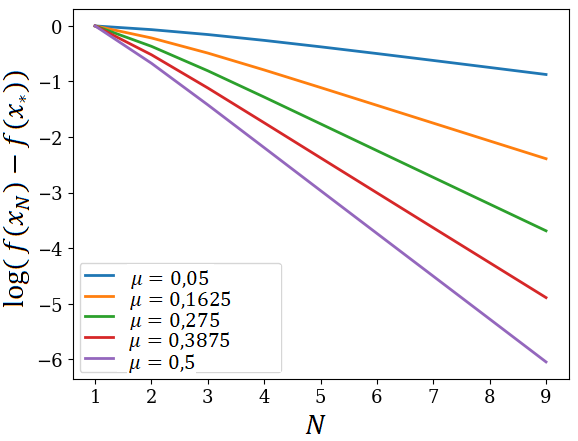
\includegraphics[width=0.5\textwidth]{linear_convergence.png}
\end{figure}

\end{frame}
%-----------------------------------------------------------------------------------------------------
\begin{frame}{Результат проверки гипотезы}
\begin{center}

 $f(x_N) - f(x_{\star}) = O\left(\left(\frac{1 - \left(\frac{\mu}{L}\right)^{\alpha(\varepsilon)}}{1 + \left(\frac{\mu}{L}\right)^{\alpha(\varepsilon)}}\right)^N\right),  \
   \alpha|_{\varepsilon = 0} = \frac12, \ \alpha|_{\varepsilon = 1} = 1$ \\ 
\end{center}
\begin{figure}
\caption{График зависимости $\alpha(\varepsilon)$. При нулевом шуме, сходимость как у ускоренных методов (NAG, HB). При больших шумах сходимость как у GD}
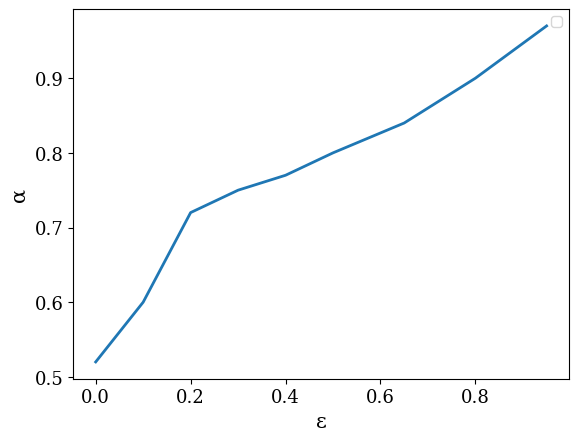
\includegraphics[width=0.6\textwidth]{main_res__of_gfom.png}
\end{figure}
\end{frame}



%-----------------------------------


%----------------------------------------------------------------------------------------------------------

%----------------------------------------------------------------------------------------------------------

%----------------------------------------------------------------------------------------------------------
\begin{frame}{Заключение}
     \begin{block}{Результаты}
     \begin{itemize}
         \item предложена гипотеза сходимости жадного алгоритма оптимизации первого порядка в случае, когда градиенты известны лишь с некоторой погрешностью
         \item численные результаты не противоречат гипотезе
     \end{itemize}
     \end{block}
     \begin{block}{Планы}
     \begin{itemize}
         \item теоретическое доказательство полученных экспериментальных результатов
     \end{itemize}
     \end{block}
 \end{frame}
%----------------------------------------------------------------------------------------------------------
%-----------------------------------



\end{document} 
